\section{Requirements Analysis and Use-Case Modeling}
\label{sec:requirements}

\safesubsection{Stakeholders and System Actors}
\label{subsec:stakeholders-actors}
Stakeholders include all campus groups affected by the mobility service (\Cref{tab:stakeholders}), whereas \textbf{system actors} strictly denote external entities that interact directly across the software boundary (\Cref{tab:actors}). Primary actor \textbf{A1 (User)} is specialized into \textbf{A1a (Student/Renter)} and \textbf{A1b (Private EV Owner)}; field technicians (\texttt{S4}) are indirect stakeholders whose repair and dispatch tasks are recorded by \textbf{A2 (Operator)}.

\begin{table}[H]
  \centering
  \singlespacing\footnotesize
  \caption{Stakeholder Analysis (\texttt{S1}--\texttt{S6}) for the VNU-HCM Smart E-Mobility Hub}
  \label{tab:stakeholders}
  \renewcommand{\arraystretch}{1.24}
  \begin{tabularx}{\textwidth}{|C{1.0cm}|L{3.1cm}|L{3.2cm}|Y|L{2.8cm}|}
    \hline
    \rowcolor{tblHeader}
    \textbf{ID} & \textbf{Stakeholder} & \textbf{Role} & \textbf{Main Goals} & \textbf{Interaction} \\
    \hline
    \texttt{S1} & Shared-EV Student Commuter & Commutes between Metro Line 1, campuses, and dorms & Locate nearby charged EVs; guarantee pickup hold and return space. & \textbf{Direct}\newline(Actor \texttt{A1a} Renter) \\
    \hline
    \texttt{S2} & Private-EV Student Owner & Rides personal e-bike or e-scooter to campus & Reserve Zone C parking bays and conflict-free charging slots in advance. & \textbf{Direct}\newline(Actor \texttt{A1b} Private) \\
    \hline
    \texttt{S3} & Mobility Hub Operator & Supervises network and makes operational decisions & Early overload warning; approve bookings; prioritize charging; dispatch EVs; resolve incidents. & \textbf{Direct}\newline(Actor \texttt{A2} Console) \\
    \hline
    \texttt{S4} & Field Maintenance \& Dispatch Crew & Repairs faulty hardware and relocates EVs & Receive clear hub, slot, and unit IDs for repairs and transfers. & \textbf{Indirect}\newline(via Actor \texttt{A2}) \\
    \hline
    \texttt{S5} & VNU-HCM Urban Area Management & Sets campus e-mobility governance policies & Efficient charger/parking utilization, reduced gate congestion, commuter safety. & \textbf{Indirect}\newline(encoded in rules) \\
    \hline
    \texttt{S6} & Campus \& Dormitory Administrators & Provide physical hub sites and electrical supply & Prevent hub overflow onto walkways and avoid local power overload. & \textbf{Indirect}\newline(capacity limits) \\
    \hline
  \end{tabularx}
\end{table}

\begin{table}[H]
  \centering
  \singlespacing\footnotesize
  \caption{External System Actors (\texttt{A1}--\texttt{A3}) Derived from the System Boundary}
  \label{tab:actors}
  \renewcommand{\arraystretch}{1.24}
  \begin{tabularx}{\textwidth}{|C{1.1cm}|L{3.4cm}|C{2.1cm}|Y|}
    \hline
    \rowcolor{tblHeader}
    \textbf{ID} & \textbf{Actor Name} & \textbf{Actor Type} & \textbf{Direct System Interactions} \\
    \hline
    \texttt{A1} & User (\texttt{A1a} Student/Renter; \texttt{A1b} Private EV Owner) & Primary & Views live hub map and resource counts, searches shared EVs, reserves/cancels/picks up/returns EVs (\texttt{A1a}), or views/books Zone C parking and schedules smart charging (\texttt{A1b}). \\
    \hline
    \texttt{A2} & Hub Operator & Primary & Monitors network KPIs and utilization, approves/rejects bookings, manages 3-zone parking, sets charging queue priorities, records/closes incidents, redistributes EVs, and runs What-If scenarios. \\
    \hline
    \texttt{A3} & IoT Sensor / Simulated Data Source & Supporting & Sends timestamped status reports (vehicle SoC, slot occupancy, charger status) via REST telemetry endpoints. \\
    \hline
  \end{tabularx}
\end{table}

\safesubsection{Functional Requirements}
\label{subsec:functional-requirements}
Following ISO/IEC/IEEE 29148 \cite{iso29148}, \Cref{tab:fr-student,tab:fr-operator} define the 18 verifiable functional requirements (\texttt{FR-01}--\texttt{FR-18}).

\begin{table}[H]
  \centering
  \singlespacing\footnotesize
  \caption{Functional Requirements --- Part 1: Student Workflows (\texttt{FR-01}--\texttt{FR-10})}
  \label{tab:fr-student}
  \renewcommand{\arraystretch}{1.22}
  \begin{tabularx}{\textwidth}{|C{1.4cm}|L{2.7cm}|Y|}
    \hline
    \rowcolor{tblHeader}
    \textbf{ID} & \textbf{Category} & \textbf{Requirement Specification} \\
    \hline
    \texttt{FR-01} & Hub Discovery & Show each Mobility Hub on the live map and card list with available rental EVs, free parking bays, and available charging ports. \\
    \hline
    \texttt{FR-02} & Vehicle Search & Allow \texttt{A1} to filter hubs and shared EVs by keyword, hub, and vehicle type, showing availability, battery SoC (\%), range (km), and VND rate. \\
    \hline
    \texttt{FR-03} & Private EV Mode & Allow \texttt{A1} to view parking and charging availability and manage isolated private EV profiles without invoking shared rental actions. \\
    \hline
    \texttt{FR-04} & Vehicle Booking & Create a \texttt{PENDING} vehicle reservation only if \texttt{A1} has no open rental, $\text{SoC} \ge 20\%$, and the time window is non-overlapping; otherwise reject with reason. \\
    \hline
    \texttt{FR-05} & Approval \& QR & Allow \texttt{A2} to approve (\texttt{CONFIRMED}) or reject (\texttt{CANCELLED}) pending bookings, and mark reservation \texttt{ACTIVE} / vehicle \texttt{IN\_\allowbreak USE} upon \texttt{A1} optical QR pickup. \\
    \hline
    \texttt{FR-06} & Vehicle Return & Accept vehicle return only when the destination hub has a free \texttt{SHARED\_\allowbreak EV} or \texttt{UNIVERSAL} bay, docking the EV, syncing hub status, and closing as \texttt{COMPLETED}. \\
    \hline
    \texttt{FR-07} & Cancel \& Expiry & Release held vehicle/slot resources if \texttt{A1} cancels while \texttt{PENDING} (\texttt{STUDENT\_\allowbreak CANCELLED}), declines pickup (\texttt{STUDENT\_\allowbreak DECLINED}), or exceeds the 15-minute hold (\texttt{EXPIRED}). \\
    \hline
    \texttt{FR-08} & Parking Booking & Reserve a Zone C bay (\texttt{PRIVATE\_\allowbreak EV} or \texttt{UNIVERSAL}) via \texttt{AUTO} free-bay assignment or explicit choice when capacity exists; reject when all compatible bays are booked. \\
    \hline
    \texttt{FR-09} & Charger Booking & Schedule charging (\texttt{SCHEDULED}, target $100\%$) on any free operational port during the interval, supporting concurrent student bookings when 2+ ports are free. \\
    \hline
    \texttt{FR-10} & Charging Queue & Place charging requests into a \texttt{QUEUED} priority waitlist whenever all operational chargers at the hub are locked during the requested interval. \\
    \hline
  \end{tabularx}
\end{table}

\begin{table}[H]
  \centering
  \singlespacing\footnotesize
  \caption{Functional Requirements --- Part 2: Operator, Simulation \& Telemetry (\texttt{FR-11}--\texttt{FR-18})}
  \label{tab:fr-operator}
  \renewcommand{\arraystretch}{1.22}
  \begin{tabularx}{\textwidth}{|C{1.4cm}|L{2.7cm}|Y|}
    \hline
    \rowcolor{tblHeader}
    \textbf{ID} & \textbf{Category} & \textbf{Requirement Specification} \\
    \hline
    \texttt{FR-11} & Network Monitor & Allow \texttt{A2} to monitor live network KPIs, hub utilization ratios, 3-zone parking occupancy, active chargers, and pending approval queues. \\
    \hline
    \texttt{FR-12} & Smart Priority & Allow \texttt{A2} to set waitlist priority (\texttt{URGENT}, \texttt{HIGH}, \texttt{NORMAL}, \texttt{LOW}) and execute \texttt{Plug-in}, \texttt{Unplug}, and \texttt{Swap} across the 2-table charging console. \\
    \hline
    \texttt{FR-13} & Incident Isolate & Require \texttt{A2} to select an affected unit when logging an incident, immediately marking it \texttt{OUT\_\allowbreak OF\_\allowbreak SERVICE} (or \texttt{MAINTENANCE}) and blocking new bookings. \\
    \hline
    \texttt{FR-14} & Incident Close & Allow \texttt{A2} to assign incidents (\texttt{IN\_\allowbreak PROGRESS}) and restore the isolated resource to operational availability only upon closing with repair notes. \\
    \hline
    \texttt{FR-15} & Fleet Dispatch & Allow \texttt{A2} to redistribute \texttt{AVAILABLE} shared EVs (excluding private EVs) slot-to-slot when destination bays are free, updating both hubs atomically. \\
    \hline
    \texttt{FR-16} & What-If Sandbox & Execute What-If scenarios on an isolated in-memory copy of live operational state without modifying live reservations, vehicles, or chargers. \\
    \hline
    \texttt{FR-17} & Recommendations & Generate ranked coordination recommendations from simulated impact indicators and apply an action to live state only after \texttt{A2} confirmation and revalidation. \\
    \hline
    \texttt{FR-18} & Telemetry Ingest & Update vehicle, slot, and charger states on valid \texttt{A3} telemetry reports while rejecting invalid payloads and preserving the last valid state. \\
    \hline
  \end{tabularx}
\end{table}

\safesubsection{Non-Functional Requirements}
\label{subsec:non-functional-requirements}
\Cref{tab:nfr} specifies eight measurable Non-Functional Requirements across key quality attributes.

\begin{table}[H]
  \centering
  \singlespacing\footnotesize
  \caption{Concrete and Verifiable Non-Functional Requirements (\texttt{NFR-01}--\texttt{NFR-08})}
  \label{tab:nfr}
  \renewcommand{\arraystretch}{1.22}
  \begin{tabularx}{\textwidth}{|C{1.5cm}|L{2.8cm}|Y|}
    \hline
    \rowcolor{tblHeader}
    \textbf{ID} & \textbf{Quality Attribute} & \textbf{Measurable Criterion} \\
    \hline
    \texttt{NFR-01} & API Performance & REST read/write endpoints respond in $\le 500\text{ ms}$ (p95) under 50 concurrent campus users on local/LAN deployment. \\
    \hline
    \texttt{NFR-02} & Simulation Speed & Discrete-time What-If runs up to 20 hubs, 200 EVs, and 120 simulated minutes complete in $\le 3\text{ s}$ ($30\text{ s}$ hard cap). \\
    \hline
    \texttt{NFR-03} & Concurrency Safety & Zero double-bookings or negative slot counts under concurrent requests via InnoDB \texttt{SELECT ... FOR UPDATE} row locks. \\
    \hline
    \texttt{NFR-04} & Sandbox Isolation & Running any What-If scenario causes $0$ row modifications across all live MySQL operational tables. \\
    \hline
    \texttt{NFR-05} & Security \& RBAC & Protected routes enforce HS256 JWT verification, \texttt{403 FORBIDDEN} role checks, and 100\% parameterized SQL statements. \\
    \hline
    \texttt{NFR-06} & Fault Tolerance & Malformed inputs reject pre-transaction with structured \texttt{400/422} codes; DB deadlocks map to \texttt{409} without leaking SQL text. \\
    \hline
    \texttt{NFR-07} & Mobile Usability & Responsive desktop ($1440\text{ px}$) and mobile portrait ($375\text{ px}$ LAN) layouts with zero horizontal overflow, Dark/Light themes, and $4\text{ s}$ live sync. \\
    \hline
    \texttt{NFR-08} & Maintainability & Modular domain services aligned with OpenAPI 3.0 REST contract specifications and centralized state-transition guards. \\
    \hline
  \end{tabularx}
\end{table}

\safesubsection{Business Rules and Operational Constraints}
\label{subsec:business-rules}
\Cref{tab:business-rules} formalizes the seven core domain rules enforced across all backend services.

\begin{table}[H]
  \centering
  \singlespacing\footnotesize
  \caption{Core Domain Business Rules and Operational Constraints (\texttt{BR-01}--\texttt{BR-07})}
  \label{tab:business-rules}
  \renewcommand{\arraystretch}{1.22}
  \begin{tabularx}{\textwidth}{|C{1.4cm}|L{3.4cm}|Y|}
    \hline
    \rowcolor{tblHeader}
    \textbf{Rule} & \textbf{Rule Name} & \textbf{Enforced Operational Invariant} \\
    \hline
    \texttt{BR-01} & Single Open Rental Mutex & Each \texttt{A1} account may hold at most one open vehicle booking (\texttt{PENDING}, \texttt{CONFIRMED}, or \texttt{ACTIVE}), serialized by locking \texttt{users} first. \\
    \hline
    \texttt{BR-02} & Minimum Safe Battery & Shared EVs with $\text{battery\_level} < 20\%$ cannot be reserved or picked up and are prioritized for hub charging. \\
    \hline
    \texttt{BR-03} & 5-Stage Role-Safe Lifecycle & Bookings start at \texttt{PENDING}; only \texttt{A2} approves (\texttt{CONFIRMED}) or rejects (\texttt{OPERATOR\_\allowbreak REJECTED}); customer cancel always logs \texttt{STUDENT\_\allowbreak CANCELLED} / \texttt{STUDENT\_\allowbreak DECLINED}; holds expire after 15 minutes (\texttt{EXPIRED}). \\
    \hline
    \texttt{BR-04} & 3-Zone Parking Isolation & Zone A (\texttt{SHARED\_\allowbreak EV}) accepts only campus rental EVs; private customer EVs use Zone C (\texttt{PRIVATE\_\allowbreak EV}/\allowbreak\texttt{UNIVERSAL}) and are excluded from operator fleet dispatch. \\
    \hline
    \texttt{BR-05} & Time-Slot Lock + Waitlist & Scheduled charging locks its port against preemption; concurrent students receive distinct free ports in \texttt{AUTO} mode until all hub ports are busy, after which requests enter \texttt{QUEUED} (\texttt{URGENT > HIGH > NORMAL > LOW}, target $100\%$). \\
    \hline
    \texttt{BR-06} & Dynamic Hub Saturation & Hub status updates atomically on slot changes (unless in \texttt{MAINTENANCE}): $\ge 100\% \Rightarrow \texttt{FULL}$, $\ge 80\% \Rightarrow \texttt{NEAR\_\allowbreak FULL}$, $< 80\% \Rightarrow \texttt{ACTIVE}$. \\
    \hline
    \texttt{BR-07} & Mandatory Unit Isolation & Incidents must reference a concrete unit, immediately setting it \texttt{OUT\_\allowbreak OF\_\allowbreak SERVICE} / \texttt{MAINTENANCE} until closed with repair notes. \\
    \hline
  \end{tabularx}
\end{table}

\safesubsection{Use-Case Diagrams}
\label{subsec:use-case-diagrams}
Following UML 2.5 guidelines \cite{uml25} and avoiding a single cluttered diagram, the 18 primary use cases (\texttt{UC01}--\texttt{UC18}) and 4 included system sub-use-cases (\texttt{UC04a, UC13a, UC15a, UC16a}) are organized into four monochrome diagrams: Student discovery and reservation (\Cref{fig:uc-s1}), Student pickup, return, parking, and charging (\Cref{fig:uc-s2}), Operator monitoring, incidents, dispatch, and telemetry (\Cref{fig:uc-op1}), and Operator smart charging priority and What-If simulation (\Cref{fig:uc-op2}).

\begin{figure}[H]
  \centering
  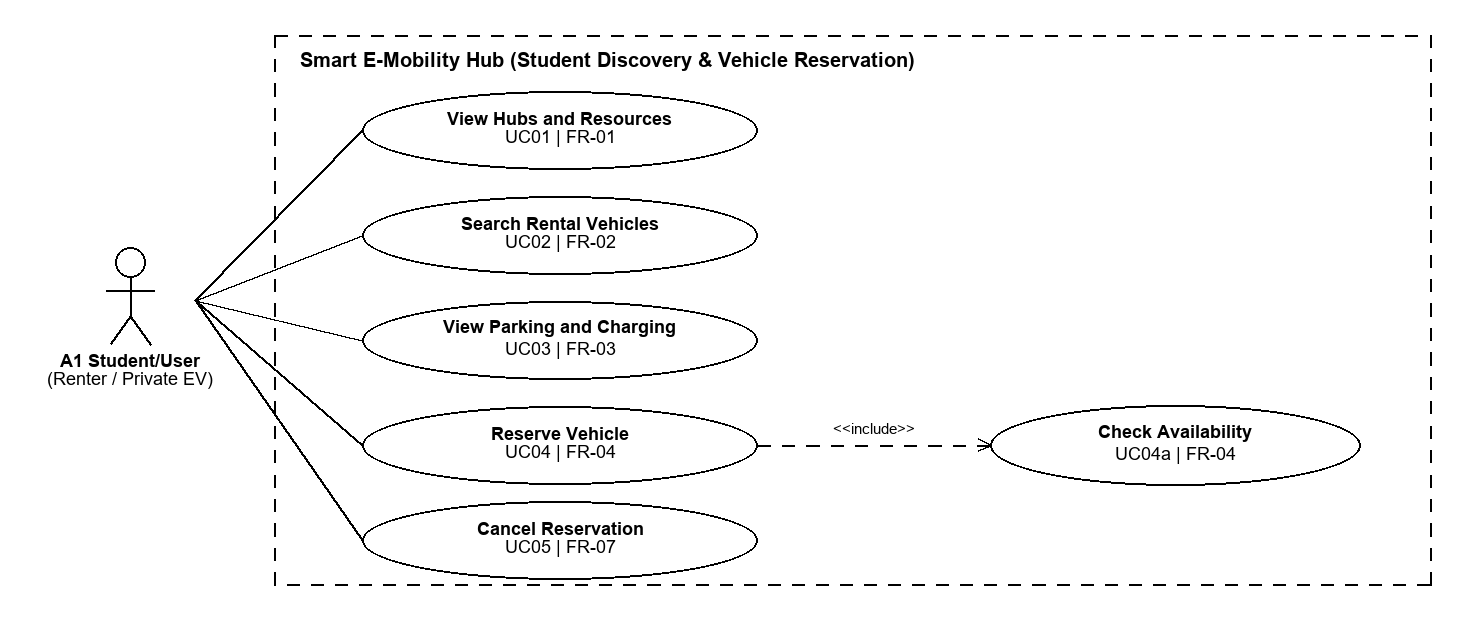
\includegraphics[width=0.88\linewidth]{graphics/diagrams/fig2_1_uc_student_search.png}
  \caption{Use-Case Diagram 1 --- Student: Hub Discovery, Vehicle Search \& Reservation (\texttt{UC01}--\texttt{UC05, UC04a})}
  \label{fig:uc-s1}
\end{figure}

\begin{figure}[H]
  \centering
  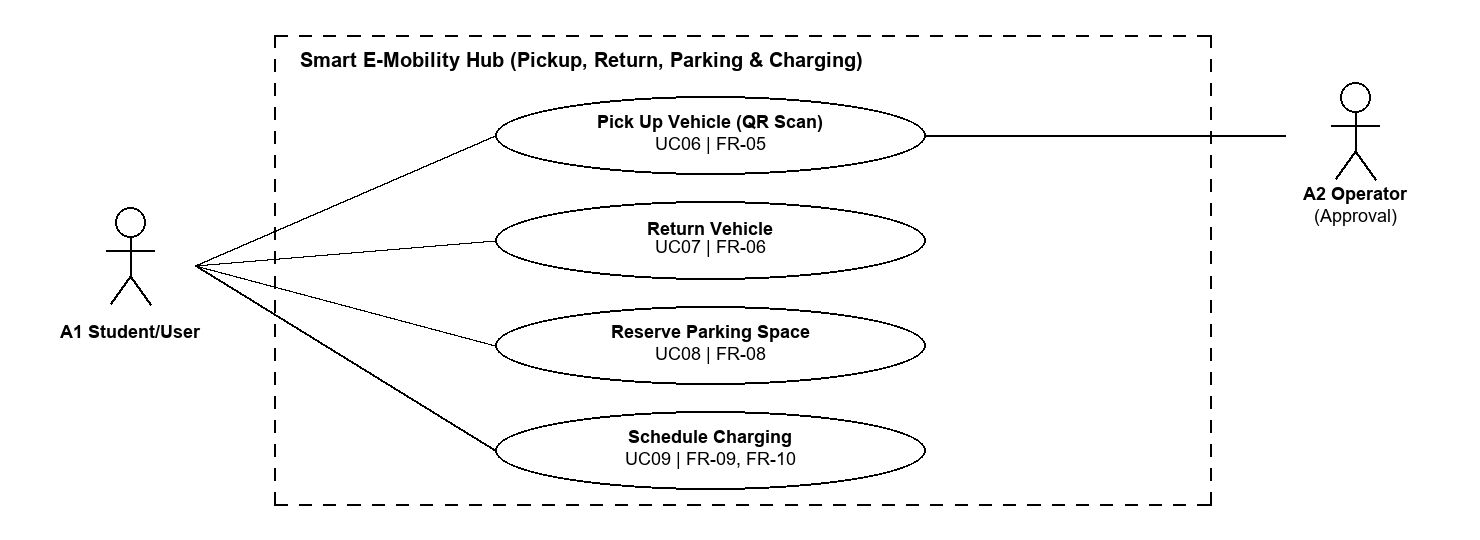
\includegraphics[width=0.88\linewidth]{graphics/diagrams/fig2_2_uc_student_ops.png}
  \caption{Use-Case Diagram 2 --- Student: QR Pickup, Return, Parking \& Smart Charging (\texttt{UC06}--\texttt{UC09})}
  \label{fig:uc-s2}
\end{figure}

\begin{figure}[H]
  \centering
  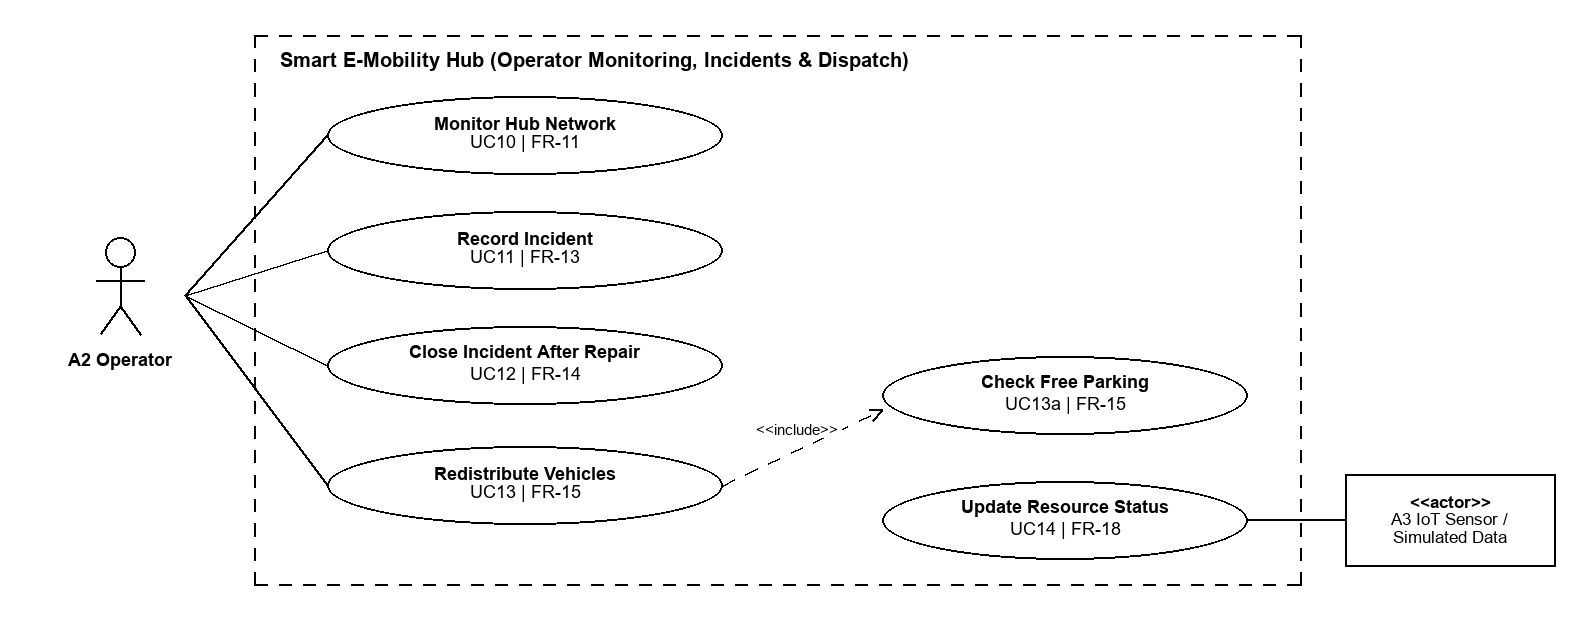
\includegraphics[width=0.90\linewidth]{graphics/diagrams/fig2_3_uc_operator_ops.png}
  \caption{Use-Case Diagram 3 --- Operator: Monitoring, Incidents, Dispatch \& Telemetry (\texttt{UC10}--\texttt{UC14, UC13a})}
  \label{fig:uc-op1}
\end{figure}

\begin{figure}[H]
  \centering
  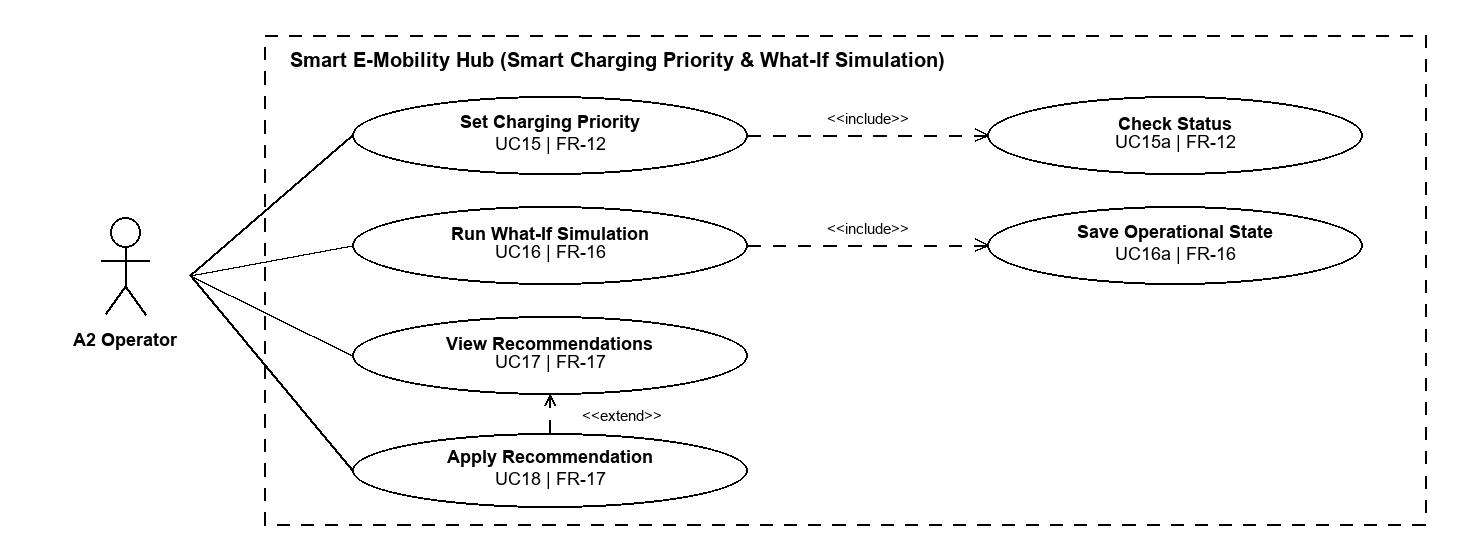
\includegraphics[width=0.88\linewidth]{graphics/diagrams/fig2_4_uc_operator_sim.png}
  \caption{Use-Case Diagram 4 --- Operator: Smart Charging Priority \& What-If Simulation (\texttt{UC15}--\texttt{UC18})}
  \label{fig:uc-op2}
\end{figure}

\safesubsection{Detailed Use-Case Specifications}
\label{subsec:use-case-specs}
\textbf{Actors and Authentication Precondition:} System actors comprise \textbf{A1 User} (specialized by \textbf{A1a Student/Renter} and \textbf{A1b Private EV Owner}), \textbf{A2 Operator}, and \textbf{A3 IoT Sensor / Simulated Data Source}. Users authenticate via campus/email credentials (with pre-configured \texttt{OPERATOR} accounts and default \texttt{USER} accounts for renters/private EV owners); authentication is a universal precondition of every use case rather than a separate domain use case. \Cref{tab:uc-catalog} indexes all 22 use cases and included sub-flows, followed by complete individual specifications in \Cref{tab:uc01,tab:uc02,tab:uc03,tab:uc04,tab:uc04a,tab:uc05,tab:uc06,tab:uc07,tab:uc08,tab:uc09,tab:uc10,tab:uc11,tab:uc12,tab:uc13,tab:uc13a,tab:uc14,tab:uc15,tab:uc15a,tab:uc16,tab:uc16a,tab:uc17,tab:uc18}.

\begin{table}[H]
  \centering
  \singlespacing\footnotesize
  \caption{Master Use-Case Catalog (\texttt{UC01}--\texttt{UC18} and Included Use Cases)}
  \label{tab:uc-catalog}
  \renewcommand{\arraystretch}{1.14}
  \begin{tabularx}{\textwidth}{|C{1.5cm}|Y|C{2.1cm}|L{2.8cm}|}
    \hline
    \rowcolor{tblHeader}
    \textbf{ID} & \textbf{Use Case} & \textbf{Actor} & \textbf{Related FR} \\
    \hline
    \texttt{UC01} & View Hubs and resources & \texttt{A1} & \texttt{FR-01} \\
    \hline
    \texttt{UC02} & Search rental vehicles & \texttt{A1} & \texttt{FR-02} \\
    \hline
    \texttt{UC03} & View parking and charging & \texttt{A1} & \texttt{FR-03} \\
    \hline
    \texttt{UC04} & Reserve vehicle & \texttt{A1} & \texttt{FR-04, FR-05} \\
    \hline
    \texttt{UC04a} & Check availability (included in \texttt{UC04}) & System & \texttt{FR-04} \\
    \hline
    \texttt{UC05} & Cancel reservation & \texttt{A1} & \texttt{FR-07} \\
    \hline
    \texttt{UC06} & Pick up vehicle & \texttt{A1} & \texttt{FR-05} \\
    \hline
    \texttt{UC07} & Return vehicle & \texttt{A1} & \texttt{FR-06} \\
    \hline
    \texttt{UC08} & Reserve parking space & \texttt{A1} & \texttt{FR-08} \\
    \hline
    \texttt{UC09} & Schedule charging & \texttt{A1} & \texttt{FR-09, FR-10} \\
    \hline
    \texttt{UC10} & Monitor Hub network & \texttt{A2} & \texttt{FR-11} \\
    \hline
    \texttt{UC11} & Record incident & \texttt{A2} & \texttt{FR-13} \\
    \hline
    \texttt{UC12} & Close incident after repair & \texttt{A2} & \texttt{FR-14} \\
    \hline
    \texttt{UC13} & Redistribute vehicles & \texttt{A2} & \texttt{FR-15} \\
    \hline
    \texttt{UC13a} & Check free parking (included in \texttt{UC13}) & System & \texttt{FR-15} \\
    \hline
    \texttt{UC14} & Update resource status & \texttt{A3} & \texttt{FR-18} \\
    \hline
    \texttt{UC15} & Set charging priority & \texttt{A2} & \texttt{FR-12} \\
    \hline
    \texttt{UC15a} & Check status (included in \texttt{UC15}) & System & \texttt{FR-12} \\
    \hline
    \texttt{UC16} & Run What-if simulation & \texttt{A2} & \texttt{FR-16} \\
    \hline
    \texttt{UC16a} & Save operational state (included in \texttt{UC16}) & System & \texttt{FR-16} \\
    \hline
    \texttt{UC17} & View recommendations & \texttt{A2} & \texttt{FR-17} \\
    \hline
    \texttt{UC18} & Apply recommendation (extends \texttt{UC17}) & \texttt{A2} & \texttt{FR-17} \\
    \hline
  \end{tabularx}
\end{table}

% --- PAIR 1: UC01 & UC02 ---
\begin{table}[H]
  \centering
  \singlespacing\footnotesize
  \caption{Use-Case Specification --- \texttt{UC01}: View Hubs and Resources}
  \label{tab:uc01}
  \renewcommand{\arraystretch}{1.13}
  \begin{tabularx}{\textwidth}{|L{2.9cm}|Y|}
    \hline
    \rowcolor{tblHeader}
    \textbf{Use-case name} & \textbf{\texttt{UC01} --- View Hubs and resources} \\
    \hline
    \textbf{Actor} & \texttt{A1} Student/User \\
    \hline
    \textbf{Description} & \texttt{A1} views each Mobility Hub on the interactive map and card list with its available rental vehicles, free parking spaces, and available charging points. \\
    \hline
    \textbf{Preconditions} & \texttt{A1} is logged in. Hub status data has been received from \texttt{A3} / live database. \\
    \hline
    \textbf{Normal Flow} & 1.\ \texttt{A1} opens the Hub list or live OpenStreetMap view.\newline
    2.\ System retrieves the current state of all four VNU-HCM Hubs.\newline
    3.\ System computes availability: available vehicles (excluding reserved, \texttt{IN\_\allowbreak USE}, low-battery charging, or \texttt{OUT\_\allowbreak OF\_\allowbreak SERVICE}); free parking $= \text{capacity} - (\text{occupied} + \text{overlapping reserved})$; available chargers $= \text{capacity} - (\text{occupied, reserved, or unavailable})$.\newline
    4.\ System displays each Hub with its saturation badge, name, and the three resource counts.\newline
    5.\ \texttt{A1} selects a Hub marker or card; 6.\ System displays detailed fleet, bay, and charger data for that Hub. \\
    \hline
    \textbf{Exceptions} & \textbf{2a.} Hub telemetry has not updated for $>30\text{ s}$: System displays the last known valid state (with last-update timestamp) and continues at step 3. \\
    \hline
    \textbf{Alternative Flows} & \textbf{5a.} \texttt{A1} does not select a specific Hub: the use case ends after step 4. \\
    \hline
    \textbf{Postconditions} & No state change. \\
    \hline
    \textbf{Related FR / NFR} & \texttt{FR-01}; \texttt{NFR-01, NFR-07} \\
    \hline
  \end{tabularx}
\end{table}

\begin{table}[H]
  \centering
  \singlespacing\footnotesize
  \caption{Use-Case Specification --- \texttt{UC02}: Search Rental Vehicles}
  \label{tab:uc02}
  \renewcommand{\arraystretch}{1.13}
  \begin{tabularx}{\textwidth}{|L{2.9cm}|Y|}
    \hline
    \rowcolor{tblHeader}
    \textbf{Use-case name} & \textbf{\texttt{UC02} --- Search rental vehicles} \\
    \hline
    \textbf{Actor} & \texttt{A1a} Student/User (rental mode) \\
    \hline
    \textbf{Description} & \texttt{A1a} searches shared e-bicycles and e-scooters by Hub, vehicle type, and operational battery/range eligibility. \\
    \hline
    \textbf{Preconditions} & \texttt{A1a} is logged in and browsing shared rental mode. \\
    \hline
    \textbf{Normal Flow} & 1.\ \texttt{A1a} opens the Hub/vehicle search and fleet filter strip.\newline
    2.\ \texttt{A1a} selects filters (Hub keyword, \texttt{Electric bike} / \texttt{Electric scooter}, battery threshold).\newline
    3.\ System queries vehicles in state \texttt{AVAILABLE} whose battery meets the safety threshold ($\text{SoC} \ge 20\%$, \texttt{BR-02}).\newline
    4.\ System displays matching vehicles with availability, current battery percentage, estimated range (km), and VND rate.\newline
    5.\ \texttt{A1a} selects a vehicle to inspect details and may proceed to \texttt{UC04}. \\
    \hline
    \textbf{Exceptions} & \textbf{2a.} Battery filter outside $0\text{--}100\%$: System rejects input with validation feedback; return to step 2.\newline
    \textbf{3a.} No vehicle matches: System shows ``No available vehicles match'' and suggests relaxing filters or trying another Hub. \\
    \hline
    \textbf{Alternative Flows} & \textbf{2b.} \texttt{A1a} leaves optional filters empty: System applies only active filters and shows all eligible vehicles with range estimates; continue step 3. \\
    \hline
    \textbf{Postconditions} & No state change. \\
    \hline
    \textbf{Related FR / NFR} & \texttt{FR-02}; \texttt{BR-02} \\
    \hline
  \end{tabularx}
\end{table}

% --- PAIR 2: UC03 & UC04 ---
\begin{table}[H]
  \centering
  \singlespacing\footnotesize
  \caption{Use-Case Specification --- \texttt{UC03}: View Parking and Charging}
  \label{tab:uc03}
  \renewcommand{\arraystretch}{1.13}
  \begin{tabularx}{\textwidth}{|L{2.9cm}|Y|}
    \hline
    \rowcolor{tblHeader}
    \textbf{Use-case name} & \textbf{\texttt{UC03} --- View parking and charging} \\
    \hline
    \textbf{Actor} & \texttt{A1b} Student/User (private-vehicle mode) \\
    \hline
    \textbf{Description} & \texttt{A1b}, riding a personal EV, views Zone C parking and charging availability and manages isolated personal EV details without invoking shared-rental actions. \\
    \hline
    \textbf{Preconditions} & \texttt{A1b} is logged in and opens Hub Services / Book Parking \& Charger mode. \\
    \hline
    \textbf{Normal Flow} & 1.\ \texttt{A1b} selects a Hub in the private-EV parking/charging workspace (and optionally edits personal EV plate/model).\newline
    2.\ System isolates the view from shared fleet rental holds.\newline
    3.\ System retrieves Zone C (\texttt{PRIVATE\_\allowbreak EV}/\texttt{UNIVERSAL}) parking bays and operational charging points of the Hub.\newline
    4.\ System displays free parking spaces, available chargers, and 7-day hourly availability; 5.\ \texttt{A1b} may continue with \texttt{UC08} or \texttt{UC09}. \\
    \hline
    \textbf{Exceptions} & \textbf{3a.} Telemetry is delayed: System shows last valid counts; continue step 4.\newline
    \textbf{4a.} Zero free parking bays and zero free chargers: System shows full status and suggests nearby VNU-HCM Hubs. \\
    \hline
    \textbf{Alternative Flows} & \textbf{5a.} \texttt{A1b} switches to compare another Hub: return to step 1. \\
    \hline
    \textbf{Postconditions} & No shared-fleet state change (personal EV profile saved per user if edited). \\
    \hline
    \textbf{Related FR / NFR} & \texttt{FR-03}; \texttt{BR-04} \\
    \hline
  \end{tabularx}
\end{table}

\begin{table}[H]
  \centering
  \singlespacing\footnotesize
  \caption{Use-Case Specification --- \texttt{UC04}: Reserve Vehicle}
  \label{tab:uc04}
  \renewcommand{\arraystretch}{1.13}
  \begin{tabularx}{\textwidth}{|L{2.9cm}|Y|}
    \hline
    \rowcolor{tblHeader}
    \textbf{Use-case name} & \textbf{\texttt{UC04} --- Reserve vehicle} \\
    \hline
    \textbf{Actor} & \texttt{A1a} Student/User (primary); \texttt{A2} Operator (booking approval) \\
    \hline
    \textbf{Description} & \texttt{A1a} reserves a shared EV for a 7-day time window at a Hub (including \texttt{UC04a} Check availability), followed by \texttt{A2} approval into a 15-minute pickup hold. \\
    \hline
    \textbf{Preconditions} & \texttt{A1a} is logged in. An eligible vehicle ($\text{SoC} \ge 20\%$) was selected through \texttt{UC02}. \\
    \hline
    \textbf{Normal Flow} & 1.\ \texttt{A1a} selects a vehicle and chooses \textit{Reserve} with a start/end window.\newline
    2.\ System locks \texttt{users} (\texttt{FOR UPDATE}) and checks \texttt{A1a} holds no other open vehicle booking (\texttt{BR-01}).\newline
    3.\ System executes \texttt{UC04a} Check availability under row lock.\newline
    4.\ System creates reservation (\texttt{PENDING}) and holds the vehicle; upon \texttt{A2} clicking \textit{Approve}, status transitions to \texttt{CONFIRMED} and starts the 15-minute pickup deadline timer.\newline
    5.\ System displays confirmation (vehicle, Hub, time window, VND estimate, pickup deadline) and auto-syncs within $4\text{ s}$. \\
    \hline
    \textbf{Exceptions} & \textbf{2a.} \texttt{A1a} already holds an open rental: rejected (\texttt{409 USER\_\allowbreak HAS\_\allowbreak ACTIVE\_\allowbreak RENTAL}); \texttt{A1a} may cancel via \texttt{UC05}.\newline
    \textbf{3a.} \texttt{UC04a} returns invalid (low battery or overlap) or concurrent request locked the EV first: rejected (\texttt{409}); return to step 1/2.\newline
    \textbf{4a.} \texttt{A2} rejects request: reservation becomes \texttt{CANCELLED} (\texttt{OPERATOR\_\allowbreak REJECTED}) and EV returns to \texttt{AVAILABLE}. \\
    \hline
    \textbf{Alternative Flows} & None. \\
    \hline
    \textbf{Postconditions} & Reservation is recorded and the vehicle cannot be double-booked for the overlapping window. \\
    \hline
    \textbf{Related FR / NFR} & \texttt{FR-04, FR-05}; \texttt{NFR-03} \\
    \hline
  \end{tabularx}
\end{table}

% --- PAIR 3: UC04a & UC05 ---
\begin{table}[H]
  \centering
  \singlespacing\footnotesize
  \caption{Use-Case Specification --- \texttt{UC04a}: Check Availability (Included in \texttt{UC04})}
  \label{tab:uc04a}
  \renewcommand{\arraystretch}{1.13}
  \begin{tabularx}{\textwidth}{|L{2.9cm}|Y|}
    \hline
    \rowcolor{tblHeader}
    \textbf{Use-case name} & \textbf{\texttt{UC04a} --- Check availability (included in \texttt{UC04})} \\
    \hline
    \textbf{Actor} & System (no external actor) \\
    \hline
    \textbf{Description} & Verifies transactionally that the selected vehicle remains operational, adequately charged, and free of overlapping bookings for the requested window. \\
    \hline
    \textbf{Preconditions} & \texttt{UC04} has supplied a validated vehicle ID and $[t_{\text{start}}, t_{\text{end}})$ window. \\
    \hline
    \textbf{Normal Flow} & 1.\ System locks and reads the current \texttt{vehicles} row and active \texttt{reservations}.\newline
    2.\ System verifies the Hub is not \texttt{MAINTENANCE}, vehicle is \texttt{AVAILABLE}, and $\text{battery\_level} \ge 20\%$.\newline
    3.\ System verifies $[t_{\text{start}}, t_{\text{end}})$ overlaps zero \texttt{PENDING}, \texttt{CONFIRMED}, or \texttt{ACTIVE} reservations of that vehicle.\newline
    4.\ System returns \texttt{valid} to \texttt{UC04}. \\
    \hline
    \textbf{Exceptions} & \textbf{2a, 3a.} Any check fails: System returns \texttt{invalid} with the exact error code (\texttt{BATTERY\_\allowbreak TOO\_\allowbreak LOW} or \texttt{VEHICLE\_\allowbreak TIME\_\allowbreak SLOT\_\allowbreak BOOKED}) to \texttt{UC04}, which aborts creation. \\
    \hline
    \textbf{Alternative Flows} & None. \\
    \hline
    \textbf{Postconditions} & No state change within \texttt{UC04a} itself. \\
    \hline
    \textbf{Related FR / NFR} & \texttt{FR-04}; \texttt{NFR-03} \\
    \hline
  \end{tabularx}
\end{table}

\begin{table}[H]
  \centering
  \singlespacing\footnotesize
  \caption{Use-Case Specification --- \texttt{UC05}: Cancel Reservation}
  \label{tab:uc05}
  \renewcommand{\arraystretch}{1.13}
  \begin{tabularx}{\textwidth}{|L{2.9cm}|Y|}
    \hline
    \rowcolor{tblHeader}
    \textbf{Use-case name} & \textbf{\texttt{UC05} --- Cancel reservation} \\
    \hline
    \textbf{Actor} & \texttt{A1} Student/User (or System timer on hold expiry) \\
    \hline
    \textbf{Description} & \texttt{A1} cancels a vehicle or parking reservation before pickup/check-in, or the system automatically releases a reservation when the 15-minute pickup hold expires. \\
    \hline
    \textbf{Preconditions} & Reservation is in \texttt{PENDING} or \texttt{CONFIRMED} state and has not been picked up. \\
    \hline
    \textbf{Normal Flow} & 1.\ \texttt{A1} opens the active reservation and selects \textit{Cancel}.\newline
    2.\ System prompts for confirmation; 3.\ \texttt{A1} confirms cancellation.\newline
    4.\ System sets reservation status to \texttt{CANCELLED} with role-safe student attribution (\texttt{STUDENT\_\allowbreak CANCELLED} or \texttt{STUDENT\_\allowbreak DECLINED}, never \texttt{OPERATOR\_\allowbreak REJECTED}) and restores any held vehicle/slot to \texttt{AVAILABLE}/\texttt{FREE}.\newline
    5.\ System displays the updated cancellation badge. \\
    \hline
    \textbf{Exceptions} & \textbf{2a.} Reservation is already \texttt{ACTIVE} (picked up), \texttt{COMPLETED}, or \texttt{EXPIRED}: System rejects cancellation (\texttt{409 INVALID\_\allowbreak STATE\_\allowbreak TRANSITION}) with reason. \\
    \hline
    \textbf{Alternative Flows} & \textbf{3a.} \texttt{A1} dismisses confirmation: no state change; use case ends.\newline
    \textbf{1a (Expiry):} No pickup occurs within 15 minutes after the scheduled start; system marks reservation \texttt{EXPIRED}, restores EV to \texttt{AVAILABLE}, and updates \texttt{A1}'s view. \\
    \hline
    \textbf{Postconditions} & Held vehicle or bay is \texttt{AVAILABLE}/\texttt{FREE} again for other campus users. \\
    \hline
    \textbf{Related FR / NFR} & \texttt{FR-07}; \texttt{BR-03} \\
    \hline
  \end{tabularx}
\end{table}

% --- PAIR 4: UC06 & UC07 ---
\begin{table}[H]
  \centering
  \singlespacing\footnotesize
  \caption{Use-Case Specification --- \texttt{UC06}: Pick Up Vehicle}
  \label{tab:uc06}
  \renewcommand{\arraystretch}{1.13}
  \begin{tabularx}{\textwidth}{|L{2.9cm}|Y|}
    \hline
    \rowcolor{tblHeader}
    \textbf{Use-case name} & \textbf{\texttt{UC06} --- Pick up vehicle} \\
    \hline
    \textbf{Actor} & \texttt{A1a} Student/User \\
    \hline
    \textbf{Description} & \texttt{A1a} unlocks and confirms pickup of an operator-approved vehicle at the designated Hub via optical QR scan. \\
    \hline
    \textbf{Preconditions} & Reservation is \texttt{CONFIRMED} for this \texttt{A1a}, not expired, and \texttt{A1a} is at the designated Hub rack. \\
    \hline
    \textbf{Normal Flow} & 1.\ \texttt{A1a} opens Pickup \& Return, launches the Optical QR Scanner, and scans/confirms the vehicle QR code.\newline
    2.\ System validates the Hub, ownership, non-expiry, and \texttt{CONFIRMED} state.\newline
    3.\ System sets reservation to \texttt{ACTIVE}, sets vehicle to \texttt{IN\_\allowbreak USE}, vacates the origin parking slot to \texttt{FREE}, and recalculates Hub status.\newline
    4.\ System starts the live elapsed ride timer and displays active trip telemetry. \\
    \hline
    \textbf{Exceptions} & \textbf{2a.} Reservation is still \texttt{PENDING}: rejected (\texttt{409 AWAITING\_\allowbreak OPERATOR\_\allowbreak APPROVAL}).\newline
    \textbf{2b.} Reservation expired, cancelled, wrong Hub, or owned by another user: rejected (\texttt{403/409}) with specific reason; \texttt{A1a} may start \texttt{UC02}. \\
    \hline
    \textbf{Alternative Flows} & None. \\
    \hline
    \textbf{Postconditions} & Vehicle is \texttt{IN\_\allowbreak USE}, origin slot is \texttt{FREE}, and hold expiry timer stops. \\
    \hline
    \textbf{Related FR / NFR} & \texttt{FR-05}; \texttt{NFR-03, NFR-07} \\
    \hline
  \end{tabularx}
\end{table}

\begin{table}[H]
  \centering
  \singlespacing\footnotesize
  \caption{Use-Case Specification --- \texttt{UC07}: Return Vehicle}
  \label{tab:uc07}
  \renewcommand{\arraystretch}{1.13}
  \begin{tabularx}{\textwidth}{|L{2.9cm}|Y|}
    \hline
    \rowcolor{tblHeader}
    \textbf{Use-case name} & \textbf{\texttt{UC07} --- Return vehicle} \\
    \hline
    \textbf{Actor} & \texttt{A1a} Student/User \\
    \hline
    \textbf{Description} & \texttt{A1a} returns an active rental EV at a chosen Hub; the system verifies free bay capacity, docks the EV, and updates its post-trip state from battery SoC. \\
    \hline
    \textbf{Preconditions} & Reservation is \texttt{ACTIVE} (picked up) and the vehicle is \texttt{IN\_\allowbreak USE}. \\
    \hline
    \textbf{Normal Flow} & 1.\ \texttt{A1a} selects \textit{Return vehicle} and chooses a destination Hub.\newline
    2.\ System locks destination Hub slots and checks for $\ge 1$ \texttt{FREE} \texttt{SHARED\_\allowbreak EV} or \texttt{UNIVERSAL} parking bay.\newline
    3.\ System evaluates post-trip battery SoC and docks the vehicle into the free bay (\texttt{OCCUPIED}, occupancy $+1$).\newline
    4.\ System closes the reservation as \texttt{COMPLETED} and sets the vehicle to \texttt{AVAILABLE} if $\text{SoC} \ge 20\%$, otherwise flags it for hub charging.\newline
    5.\ System syncs Hub saturation and displays the completed ride \& VND fee summary. \\
    \hline
    \textbf{Exceptions} & \textbf{2a.} Destination Hub is \texttt{MAINTENANCE} or has $0$ free compatible bays: rejected (\texttt{409 RETURN\_\allowbreak HUB\_\allowbreak FULL}); \texttt{A1a} selects another Hub with free capacity (return to step 1). \\
    \hline
    \textbf{Alternative Flows} & \textbf{5a.} Low post-trip SoC triggers charging request workflow (\texttt{UC09}). \\
    \hline
    \textbf{Postconditions} & Reservation is \texttt{COMPLETED} and vehicle is docked at the destination Hub. \\
    \hline
    \textbf{Related FR / NFR} & \texttt{FR-06}; \texttt{BR-02, BR-06} \\
    \hline
  \end{tabularx}
\end{table}

% --- PAIR 5: UC08 & UC09 ---
\begin{table}[H]
  \centering
  \singlespacing\footnotesize
  \caption{Use-Case Specification --- \texttt{UC08}: Reserve Parking Space}
  \label{tab:uc08}
  \renewcommand{\arraystretch}{1.13}
  \begin{tabularx}{\textwidth}{|L{2.9cm}|Y|}
    \hline
    \rowcolor{tblHeader}
    \textbf{Use-case name} & \textbf{\texttt{UC08} --- Reserve parking space} \\
    \hline
    \textbf{Actor} & \texttt{A1} Student/User (private-vehicle or customer parking mode) \\
    \hline
    \textbf{Description} & \texttt{A1} reserves a Zone C (\texttt{PRIVATE\_\allowbreak EV} / \texttt{UNIVERSAL}) parking space at a Hub for a requested time interval. \\
    \hline
    \textbf{Preconditions} & \texttt{A1} is logged in and has selected an operational Hub (\texttt{UC01} or \texttt{UC03}). \\
    \hline
    \textbf{Normal Flow} & 1.\ \texttt{A1} selects a Hub, time interval, and default \texttt{AUTO} free-space mode (or specific bay).\newline
    2.\ System locks compatible Zone C slots and overlapping reservations, computing free spaces $= \text{total} - (\text{occupied} + \text{overlapping active reservations})$.\newline
    3.\ System assigns a free compatible bay, creates the parking reservation, and reduces free capacity for that interval.\newline
    4.\ System displays the booking status and assigned bay code. \\
    \hline
    \textbf{Exceptions} & \textbf{2a.} Free spaces $\le 0$: System rejects (\texttt{409 NO\_\allowbreak PARKING\_\allowbreak AVAILABLE}) and suggests other Hubs or unshaded hours.\newline
    \textbf{3a.} Concurrent request took the last compatible bay: rejected (\texttt{409}) cleanly. \\
    \hline
    \textbf{Alternative Flows} & \textbf{2b.} After a full-interval rejection, \texttt{A1} picks an alternative time window; continue step 2. \\
    \hline
    \textbf{Postconditions} & A conflict-free Zone C parking reservation exists for the interval. \\
    \hline
    \textbf{Related FR / NFR} & \texttt{FR-08}; \texttt{NFR-03, BR-04} \\
    \hline
  \end{tabularx}
\end{table}

\begin{table}[H]
  \centering
  \singlespacing\footnotesize
  \caption{Use-Case Specification --- \texttt{UC09}: Schedule Charging}
  \label{tab:uc09}
  \renewcommand{\arraystretch}{1.13}
  \begin{tabularx}{\textwidth}{|L{2.9cm}|Y|}
    \hline
    \rowcolor{tblHeader}
    \textbf{Use-case name} & \textbf{\texttt{UC09} --- Schedule charging} \\
    \hline
    \textbf{Actor} & \texttt{A1} Student/User (rental or private-vehicle mode) \\
    \hline
    \textbf{Description} & \texttt{A1} requests a $100\%$ target-SoC charging session at a Hub; concurrent requests bind distinct free ports under \texttt{AUTO} mode or enter the Hub waitlist when full. \\
    \hline
    \textbf{Preconditions} & \texttt{A1} is logged in; Hub is operational and vehicle requires charging ($\text{current SoC} < 100\%$). \\
    \hline
    \textbf{Normal Flow} & 1.\ \texttt{A1} selects Hub, vehicle, and time window under default \texttt{AUTO} free-charger mode.\newline
    2.\ System locks Hub \texttt{charging\_\allowbreak points} and overlapping \texttt{charging\_\allowbreak requests} (\texttt{FOR UPDATE}).\newline
    3.\ System selects an operational charger not booked in $[t_{\text{start}}, t_{\text{end}})$ (enabling 2+ students to book the same hour when 2+ ports are free).\newline
    4.\ System locks the port, creates session (\texttt{SCHEDULED}), and displays port code, window, and estimated kWh/VND fee. \\
    \hline
    \textbf{Exceptions} & \textbf{2a.} Hub in \texttt{MAINTENANCE}, vehicle invalid, or target SoC $\neq 100\%$: rejected (\texttt{409/422}) with reason. \\
    \hline
    \textbf{Alternative Flows} & \textbf{3a.} Zero ports free in $[t_{\text{start}}, t_{\text{end}})$: System places the request into the Hub's waiting queue (\texttt{QUEUED}) without preempting locked bookings; assigned when a port frees (\texttt{UC15}). \\
    \hline
    \textbf{Postconditions} & Charging request exists as \texttt{SCHEDULED} or \texttt{QUEUED}; no port is double-booked. \\
    \hline
    \textbf{Related FR / NFR} & \texttt{FR-09, FR-10}; \texttt{NFR-03, BR-05} \\
    \hline
  \end{tabularx}
\end{table}

% --- PAIR 6: UC10 & UC11 ---
\begin{table}[H]
  \centering
  \singlespacing\footnotesize
  \caption{Use-Case Specification --- \texttt{UC10}: Monitor Hub Network}
  \label{tab:uc10}
  \renewcommand{\arraystretch}{1.13}
  \begin{tabularx}{\textwidth}{|L{2.9cm}|Y|}
    \hline
    \rowcolor{tblHeader}
    \textbf{Use-case name} & \textbf{\texttt{UC10} --- Monitor Hub network} \\
    \hline
    \textbf{Actor} & \texttt{A2} Operator \\
    \hline
    \textbf{Description} & \texttt{A2} monitors fleet distribution, 3-zone parking occupancy, charger status, pending approvals, and Hub utilization across the entire VNU-HCM network. \\
    \hline
    \textbf{Preconditions} & \texttt{A2} is authenticated with \texttt{OPERATOR} role. \\
    \hline
    \textbf{Normal Flow} & 1.\ \texttt{A2} opens the Operator Control Console (\textit{Overview} / \textit{Hub utilization}).\newline
    2.\ System retrieves synchronized telemetry across all Hubs simultaneously.\newline
    3.\ System renders 4 KPI cards, live map pins, 3-zone bay occupancy, charger status, and pending approval requests.\newline
    4.\ \texttt{A2} selects a Hub or resource; 5.\ System shows granular slot/unit status and open incidents. \\
    \hline
    \textbf{Exceptions} & \textbf{2a.} Telemetry source delayed $>30\text{ s}$: System retains last valid resource state and logs timestamp; continue step 3. \\
    \hline
    \textbf{Alternative Flows} & \textbf{4a.} \texttt{A2} filters by Hub or zone: view refreshes immediately.\newline
    \textbf{4b.} New status report (\texttt{UC14}) or booking arrives: dashboard auto-refreshes every $10\text{ s}$. \\
    \hline
    \textbf{Postconditions} & No state change (unless \texttt{A2} invokes an approval or check-in action). \\
    \hline
    \textbf{Related FR / NFR} & \texttt{FR-11}; \texttt{NFR-01, NFR-07} \\
    \hline
  \end{tabularx}
\end{table}

\begin{table}[H]
  \centering
  \singlespacing\footnotesize
  \caption{Use-Case Specification --- \texttt{UC11}: Record Incident}
  \label{tab:uc11}
  \renewcommand{\arraystretch}{1.13}
  \begin{tabularx}{\textwidth}{|L{2.9cm}|Y|}
    \hline
    \rowcolor{tblHeader}
    \textbf{Use-case name} & \textbf{\texttt{UC11} --- Record incident} \\
    \hline
    \textbf{Actor} & \texttt{A2} Operator \\
    \hline
    \textbf{Description} & \texttt{A2} logs a hardware/operational fault on a mandatory target vehicle or charging point, immediately isolating it from new bookings. \\
    \hline
    \textbf{Preconditions} & \texttt{A2} is logged in; target resource exists and is not already isolated under the same open fault. \\
    \hline
    \textbf{Normal Flow} & 1.\ \texttt{A2} opens \textit{Incidents}, selects Hub, target type (\texttt{Vehicle} or \texttt{Charging point}), mandatory unit ID, severity, and description.\newline
    2.\ System sets the target resource to \texttt{OUT\_\allowbreak OF\_\allowbreak SERVICE} / \texttt{MAINTENANCE} inside an InnoDB transaction.\newline
    3.\ System immediately blocks new reservations and charging sessions on that unit.\newline
    4.\ System records the incident (\texttt{OPEN}), flags any overlapping upcoming bookings for reassignment, and displays confirmation. \\
    \hline
    \textbf{Exceptions} & \textbf{1a.} No specific target unit selected: rejected (\texttt{400 VALIDATION\_\allowbreak FAILED}).\newline
    \textbf{2a.} Resource is already isolated with an active open incident: system warns \texttt{A2} and displays the existing incident. \\
    \hline
    \textbf{Alternative Flows} & \textbf{4a.} Zero upcoming bookings affected: notification step skipped; \texttt{A2} may trigger \texttt{UC13} if Hub stock drops. \\
    \hline
    \textbf{Postconditions} & Target resource is \texttt{OUT\_\allowbreak OF\_\allowbreak SERVICE} and an open incident persists until \texttt{UC12}. \\
    \hline
    \textbf{Related FR / NFR} & \texttt{FR-13}; \texttt{BR-07} \\
    \hline
  \end{tabularx}
\end{table}

% --- PAIR 7: UC12 & UC13 ---
\begin{table}[H]
  \centering
  \singlespacing\footnotesize
  \caption{Use-Case Specification --- \texttt{UC12}: Close Incident After Repair}
  \label{tab:uc12}
  \renewcommand{\arraystretch}{1.13}
  \begin{tabularx}{\textwidth}{|L{2.9cm}|Y|}
    \hline
    \rowcolor{tblHeader}
    \textbf{Use-case name} & \textbf{\texttt{UC12} --- Close incident after repair} \\
    \hline
    \textbf{Actor} & \texttt{A2} Operator \\
    \hline
    \textbf{Description} & \texttt{A2} resolves an open/assigned incident by recording field repair notes, restoring the isolated vehicle or charger to operational availability. \\
    \hline
    \textbf{Preconditions} & An \texttt{OPEN} or \texttt{IN\_\allowbreak PROGRESS} incident exists and physical repair was completed by field crew (\texttt{S4}). \\
    \hline
    \textbf{Normal Flow} & 1.\ \texttt{A2} selects the incident (optionally clicking \textit{Assign staff} $\rightarrow$ \texttt{IN\_\allowbreak PROGRESS} first) and clicks \textit{Resolve}.\newline
    2.\ \texttt{A2} enters non-empty repair result notes.\newline
    3.\ System validates the repair notes, closes the incident (\texttt{RESOLVED}/\texttt{CLOSED}), and restores the target vehicle or charging point to \texttt{AVAILABLE}.\newline
    4.\ System recalculates Hub capacity and confirms restoration. \\
    \hline
    \textbf{Exceptions} & \textbf{3a.} Repair result note is empty: System rejects closure (\texttt{400}); resource remains \texttt{OUT\_\allowbreak OF\_\allowbreak SERVICE}. \\
    \hline
    \textbf{Alternative Flows} & \textbf{2a.} Field crew reports unit unrepairable: \texttt{A2} keeps incident open and unit remains isolated. \\
    \hline
    \textbf{Postconditions} & Incident is closed and the repaired unit is selectable for new bookings again. \\
    \hline
    \textbf{Related FR / NFR} & \texttt{FR-14}; \texttt{BR-07} \\
    \hline
  \end{tabularx}
\end{table}

\begin{table}[H]
  \centering
  \singlespacing\footnotesize
  \caption{Use-Case Specification --- \texttt{UC13}: Redistribute Vehicles}
  \label{tab:uc13}
  \renewcommand{\arraystretch}{1.13}
  \begin{tabularx}{\textwidth}{|L{2.9cm}|Y|}
    \hline
    \rowcolor{tblHeader}
    \textbf{Use-case name} & \textbf{\texttt{UC13} --- Redistribute vehicles} \\
    \hline
    \textbf{Actor} & \texttt{A2} Operator \\
    \hline
    \textbf{Description} & \texttt{A2} transfers \texttt{AVAILABLE} shared rental EVs slot-to-slot between Hubs (including \texttt{UC13a} Check free parking), excluding private customer EVs. \\
    \hline
    \textbf{Preconditions} & \texttt{A2} is logged in; selected shared EVs are \texttt{AVAILABLE} at the source Hub. \\
    \hline
    \textbf{Normal Flow} & 1.\ \texttt{A2} selects source Hub, destination Hub, assigned staff, and \texttt{AVAILABLE} shared EVs paired to target Zone A / Universal bays (from \textit{Dispatch} or \texttt{UC18}).\newline
    2.\ System runs \texttt{UC13a} Check free parking under row lock.\newline
    3.\ Inside a two-phase transaction, Phase A frees source slots (\texttt{FREE}) and Phase B binds vehicles to destination Hub \& bays (\texttt{OCCUPIED}), logging \texttt{dispatch\_\allowbreak orders}.\newline
    4.\ System updates vehicle counts and saturation statuses of both Hubs simultaneously and confirms completion. \\
    \hline
    \textbf{Exceptions} & \textbf{1a.} Vehicle is reserved, \texttt{IN\_\allowbreak USE}, \texttt{OUT\_\allowbreak OF\_\allowbreak SERVICE}, or a private EV: rejected (\texttt{409/422}).\newline
    \textbf{2a.} \texttt{UC13a} reports destination Hub closed or lacking free bays: rejected (\texttt{409}); return to step 1. \\
    \hline
    \textbf{Alternative Flows} & None. \\
    \hline
    \textbf{Postconditions} & Total network fleet size is conserved; both Hubs reflect updated slot and EV counts. \\
    \hline
    \textbf{Related FR / NFR} & \texttt{FR-15}; \texttt{BR-04, BR-06} \\
    \hline
  \end{tabularx}
\end{table}

% --- PAIR 8: UC13a & UC14 ---
\begin{table}[H]
  \centering
  \singlespacing\footnotesize
  \caption{Use-Case Specification --- \texttt{UC13a}: Check Free Parking (Included in \texttt{UC13})}
  \label{tab:uc13a}
  \renewcommand{\arraystretch}{1.13}
  \begin{tabularx}{\textwidth}{|L{2.9cm}|Y|}
    \hline
    \rowcolor{tblHeader}
    \textbf{Use-case name} & \textbf{\texttt{UC13a} --- Check free parking (included in \texttt{UC13})} \\
    \hline
    \textbf{Actor} & System \\
    \hline
    \textbf{Description} & Verifies transactionally that the destination Hub is operational and has sufficient free \texttt{SHARED\_\allowbreak EV} / \texttt{UNIVERSAL} parking bays for incoming vehicles. \\
    \hline
    \textbf{Preconditions} & \texttt{UC13} has supplied destination Hub ID and transfer quantity / target slots. \\
    \hline
    \textbf{Normal Flow} & 1.\ System locks and reads the destination Hub status, Zone A/C slot states, and overlapping active parking reservations.\newline
    2.\ System computes verified free fleet-compatible bays and checks $\text{free} \ge \text{transfer count}$.\newline
    3.\ System returns \texttt{valid} (and candidate target slots) to \texttt{UC13}. \\
    \hline
    \textbf{Exceptions} & \textbf{2a.} Destination Hub in \texttt{MAINTENANCE} or free bays $<$ transfer count: returns \texttt{invalid} with reason; \texttt{UC13} rolls back. \\
    \hline
    \textbf{Alternative Flows} & None. \\
    \hline
    \textbf{Postconditions} & No state change within \texttt{UC13a}. \\
    \hline
    \textbf{Related FR / NFR} & \texttt{FR-15}; \texttt{NFR-03} \\
    \hline
  \end{tabularx}
\end{table}

\begin{table}[H]
  \centering
  \singlespacing\footnotesize
  \caption{Use-Case Specification --- \texttt{UC14}: Update Resource Status}
  \label{tab:uc14}
  \renewcommand{\arraystretch}{1.13}
  \begin{tabularx}{\textwidth}{|L{2.9cm}|Y|}
    \hline
    \rowcolor{tblHeader}
    \textbf{Use-case name} & \textbf{\texttt{UC14} --- Update resource status} \\
    \hline
    \textbf{Actor} & \texttt{A3} IoT Sensor / Simulated Data Source \\
    \hline
    \textbf{Description} & \texttt{A3} submits a telemetry status report; the system validates payload bounds and updates vehicle SoC, parking-slot state, or charger state. \\
    \hline
    \textbf{Preconditions} & \texttt{A3} client is connected and the referenced resource ID is registered. \\
    \hline
    \textbf{Normal Flow} & 1.\ \texttt{A3} sends a telemetry report (resource ID, resource type, new status/SoC value, ISO-8601 timestamp).\newline
    2.\ System validates completeness, numeric bounds (e.g.\ battery $0\text{--}100\%$), and valid enum transition.\newline
    3.\ System updates the vehicle, parking slot, or charging point record.\newline
    4.\ System recalculates Hub utilization (\texttt{syncHubStatus}) and exposes fresh metrics to \texttt{A2} (\texttt{UC10}). \\
    \hline
    \textbf{Exceptions} & \textbf{2a.} Payload malformed, out of range ($<0\%$ or $>100\%$), or unknown ID: System rejects (\texttt{400/422}), logs error, and preserves the last valid state.\newline
    \textbf{2b.} No report for $>30\text{ s}$: System retains last known valid state with its last-updated timestamp. \\
    \hline
    \textbf{Alternative Flows} & \textbf{2c.} Out-of-order reports arrive for the same unit: System retains the state carrying the latest timestamp. \\
    \hline
    \textbf{Postconditions} & Stored operational state reflects the latest valid telemetry report. \\
    \hline
    \textbf{Related FR / NFR} & \texttt{FR-18}; \texttt{NFR-01, NFR-06} \\
    \hline
  \end{tabularx}
\end{table}

% --- PAIR 9: UC15 & UC15a ---
\begin{table}[H]
  \centering
  \singlespacing\footnotesize
  \caption{Use-Case Specification --- \texttt{UC15}: Set Charging Priority}
  \label{tab:uc15}
  \renewcommand{\arraystretch}{1.13}
  \begin{tabularx}{\textwidth}{|L{2.9cm}|Y|}
    \hline
    \rowcolor{tblHeader}
    \textbf{Use-case name} & \textbf{\texttt{UC15} --- Set charging priority} \\
    \hline
    \textbf{Actor} & \texttt{A2} Operator \\
    \hline
    \textbf{Description} & \texttt{A2} sets priority levels on waiting charging sessions (including \texttt{UC15a} Check status) and assigns/swaps free charging points to the highest-priority EVs first. \\
    \hline
    \textbf{Preconditions} & \texttt{A2} is logged in; Hub has waiting charging requests (\texttt{QUEUED}) or active ports. \\
    \hline
    \textbf{Normal Flow} & 1.\ \texttt{A2} opens the 2-table \textit{Vehicle \& charging} console.\newline
    2.\ System runs \texttt{UC15a} Check status and renders Table 1 (Active Chargers) alongside Table 2 (Priority Waitlist).\newline
    3.\ \texttt{A2} updates session priority (\texttt{URGENT}, \texttt{HIGH}, \texttt{NORMAL}, \texttt{LOW}) based on battery criticality or expected demand.\newline
    4.\ System persists the priority, re-sorts the queue overriding FIFO, and binds free ports (or executes \texttt{Plug-in}/\texttt{Swap}/\texttt{Unplug}) to top-priority sessions.\newline
    5.\ System displays confirmation and updated charger bindings. \\
    \hline
    \textbf{Exceptions} & \textbf{2a.} Queue is empty: System displays empty waitlist state; use case ends.\newline
    \textbf{4a.} Zero ports currently free: Updated priority order is saved and applied as soon as a port is unplugged. \\
    \hline
    \textbf{Alternative Flows} & \textbf{3a.} Priority update is invoked automatically from a confirmed simulation recommendation (\texttt{UC18}). \\
    \hline
    \textbf{Postconditions} & Waiting sessions are ordered strictly by priority (\texttt{URGENT..LOW}, then FIFO) and free ports are assigned. \\
    \hline
    \textbf{Related FR / NFR} & \texttt{FR-12}; \texttt{BR-05} \\
    \hline
  \end{tabularx}
\end{table}

\begin{table}[H]
  \centering
  \singlespacing\footnotesize
  \caption{Use-Case Specification --- \texttt{UC15a}: Check Status (Included in \texttt{UC15})}
  \label{tab:uc15a}
  \renewcommand{\arraystretch}{1.13}
  \begin{tabularx}{\textwidth}{|L{2.9cm}|Y|}
    \hline
    \rowcolor{tblHeader}
    \textbf{Use-case name} & \textbf{\texttt{UC15a} --- Check status (included in \texttt{UC15})} \\
    \hline
    \textbf{Actor} & System \\
    \hline
    \textbf{Description} & Collects live charging-point states and queued vehicle battery/priority metrics required for smart charger assignment. \\
    \hline
    \textbf{Preconditions} & \texttt{UC15} has requested charging state for a Hub or the network. \\
    \hline
    \textbf{Normal Flow} & 1.\ System reads Hub charging points (\texttt{AVAILABLE}, \texttt{OCCUPIED}, \texttt{RESERVED}, \texttt{OUT\_\allowbreak OF\_\allowbreak SERVICE}).\newline
    2.\ System reads \texttt{QUEUED} charging requests along with current EV battery SoC, priority enum, and arrival timestamp.\newline
    3.\ System returns the consolidated dataset to \texttt{UC15}. \\
    \hline
    \textbf{Exceptions} & \textbf{1a.} A charging point is \texttt{OUT\_\allowbreak OF\_\allowbreak SERVICE} or stale: System excludes it from automatic assignment. \\
    \hline
    \textbf{Alternative Flows} & None. \\
    \hline
    \textbf{Postconditions} & No state change. \\
    \hline
    \textbf{Related FR / NFR} & \texttt{FR-12} \\
    \hline
  \end{tabularx}
\end{table}

% --- PAIR 10: UC16 & UC16a ---
\begin{table}[H]
  \centering
  \singlespacing\footnotesize
  \caption{Use-Case Specification --- \texttt{UC16}: Run What-If Simulation}
  \label{tab:uc16}
  \renewcommand{\arraystretch}{1.13}
  \begin{tabularx}{\textwidth}{|L{2.9cm}|Y|}
    \hline
    \rowcolor{tblHeader}
    \textbf{Use-case name} & \textbf{\texttt{UC16} --- Run What-if simulation} \\
    \hline
    \textbf{Actor} & \texttt{A2} Operator \\
    \hline
    \textbf{Description} & \texttt{A2} executes a hypothetical stress scenario on an isolated RAM copy of live state (including \texttt{UC16a} Save operational state) without altering live MySQL data. \\
    \hline
    \textbf{Preconditions} & \texttt{A2} is logged in; live operational state is readable. \\
    \hline
    \textbf{Normal Flow} & 1.\ \texttt{A2} opens \textit{What-if} and selects a scenario (demand surge, Hub full, charging surge, partial charger failure, or vehicle concentration).\newline
    2.\ \texttt{A2} enters parameters (target Hub, magnitude, duration, seed); 3.\ System validates parameter ranges.\newline
    4.\ System runs \texttt{UC16a} Save operational state to obtain a deep-cloned sandbox snapshot.\newline
    5.\ System steps discrete 1-minute simulated time on the copy and computes impact indicators (\texttt{I1}--\texttt{I8}).\newline
    6.\ System displays simulated metrics and generates ranked recommendations (\texttt{UC17}). \\
    \hline
    \textbf{Exceptions} & \textbf{3a.} Out-of-range parameters: rejected (\texttt{400}); return to step 2.\newline
    \textbf{5a.} Simulation fails or exceeds the $30\text{ s}$ cap: System aborts, discards the RAM copy, and leaves live data untouched. \\
    \hline
    \textbf{Alternative Flows} & \textbf{6a.} \texttt{A2} adjusts scenario parameters and re-runs; return to step 2. \\
    \hline
    \textbf{Postconditions} & Live reservations, EV locations, and charging sessions experience $0$ database writes. \\
    \hline
    \textbf{Related FR / NFR} & \texttt{FR-16}; \texttt{NFR-02, NFR-04} \\
    \hline
  \end{tabularx}
\end{table}

\begin{table}[H]
  \centering
  \singlespacing\footnotesize
  \caption{Use-Case Specification --- \texttt{UC16a}: Save Operational State (Included in \texttt{UC16})}
  \label{tab:uc16a}
  \renewcommand{\arraystretch}{1.13}
  \begin{tabularx}{\textwidth}{|L{2.9cm}|Y|}
    \hline
    \rowcolor{tblHeader}
    \textbf{Use-case name} & \textbf{\texttt{UC16a} --- Save operational state (included in \texttt{UC16})} \\
    \hline
    \textbf{Actor} & System \\
    \hline
    \textbf{Description} & Builds an isolated in-memory deep copy of live operational tables as the immutable starting baseline for What-If simulation. \\
    \hline
    \textbf{Preconditions} & \texttt{UC16} has validated scenario input parameters. \\
    \hline
    \textbf{Normal Flow} & 1.\ System reads a consistent snapshot of \texttt{hubs}, \texttt{vehicles}, \texttt{parking\_\allowbreak slots}, \texttt{charging\_\allowbreak points}, \texttt{reservations}, and \texttt{charging\_\allowbreak requests}.\newline
    2.\ System deep-clones the object graph in memory tagged as sandbox simulation state.\newline
    3.\ System returns the isolated snapshot to \texttt{UC16}. \\
    \hline
    \textbf{Exceptions} & \textbf{1a.} Snapshot read error: System aborts \texttt{UC16} cleanly and reports error to \texttt{A2}. \\
    \hline
    \textbf{Alternative Flows} & None. \\
    \hline
    \textbf{Postconditions} & Isolated memory snapshot exists; live MySQL tables remain untouched. \\
    \hline
    \textbf{Related FR / NFR} & \texttt{FR-16}; \texttt{NFR-04} \\
    \hline
  \end{tabularx}
\end{table}

% --- PAIR 11: UC17 & UC18 ---
\begin{table}[H]
  \centering
  \singlespacing\footnotesize
  \caption{Use-Case Specification --- \texttt{UC17}: View Recommendations}
  \label{tab:uc17}
  \renewcommand{\arraystretch}{1.13}
  \begin{tabularx}{\textwidth}{|L{2.9cm}|Y|}
    \hline
    \rowcolor{tblHeader}
    \textbf{Use-case name} & \textbf{\texttt{UC17} --- View recommendations} \\
    \hline
    \textbf{Actor} & \texttt{A2} Operator \\
    \hline
    \textbf{Description} & \texttt{A2} inspects ranked coordination recommendations (vehicle redistribution or charging priority promotion) produced by a completed What-If run. \\
    \hline
    \textbf{Preconditions} & A finished simulation result exists from \texttt{UC16}. \\
    \hline
    \textbf{Normal Flow} & 1.\ \texttt{A2} views the recommendation panel of the completed simulation.\newline
    2.\ System lists candidate actions (\texttt{R1}--\texttt{R4}) achieving $\ge 5\%$ composite stress reduction, all marked \texttt{Pending}.\newline
    3.\ \texttt{A2} inspects a recommendation; 4.\ System displays affected Hubs, EV count or queue priority target, and Before vs.\ After impact indicators. \\
    \hline
    \textbf{Exceptions} & \textbf{2a.} No candidate action improves network stress by $\ge 5\%$: System states that no coordination intervention is required. \\
    \hline
    \textbf{Alternative Flows} & \textbf{4a.} \texttt{A2} chooses to execute a recommendation on live state: \texttt{UC18} extends \texttt{UC17}. \\
    \hline
    \textbf{Postconditions} & No live state change; recommendations remain \texttt{Pending}. \\
    \hline
    \textbf{Related FR / NFR} & \texttt{FR-17} \\
    \hline
  \end{tabularx}
\end{table}

\begin{table}[H]
  \centering
  \singlespacing\footnotesize
  \caption{Use-Case Specification --- \texttt{UC18}: Apply Recommendation (Extends \texttt{UC17})}
  \label{tab:uc18}
  \renewcommand{\arraystretch}{1.13}
  \begin{tabularx}{\textwidth}{|L{2.9cm}|Y|}
    \hline
    \rowcolor{tblHeader}
    \textbf{Use-case name} & \textbf{\texttt{UC18} --- Apply recommendation (extends \texttt{UC17})} \\
    \hline
    \textbf{Actor} & \texttt{A2} Operator \\
    \hline
    \textbf{Description} & \texttt{A2} explicitly confirms a \texttt{Pending} recommendation, prompting live-state revalidation and transactional execution via \texttt{UC13} or \texttt{UC15}. \\
    \hline
    \textbf{Preconditions} & A \texttt{Pending} recommendation is selected in \texttt{UC17}. \\
    \hline
    \textbf{Normal Flow} & 1.\ \texttt{A2} clicks \textit{Apply} on the selected recommendation.\newline
    2.\ System displays the concrete live actions to be taken and requests explicit confirmation; 3.\ \texttt{A2} confirms.\newline
    4.\ System revalidates all domain guards against current live MySQL state (free destination bays, charger availability, shared EVs still \texttt{AVAILABLE}).\newline
    5.\ System executes the action transactionally via \texttt{UC13} (redistribution) or \texttt{UC15} (charging priority), marks the recommendation \texttt{Applied}, and displays the result. \\
    \hline
    \textbf{Exceptions} & \textbf{3a.} \texttt{A2} declines confirmation: zero live writes; recommendation stays \texttt{Pending}.\newline
    \textbf{4a.} Live Hub state changed since simulation snapshot causing a rule check to fail: System rejects execution (\texttt{409 STALE\_\allowbreak RECOMMENDATION}) and marks the recommendation outdated. \\
    \hline
    \textbf{Alternative Flows} & None. \\
    \hline
    \textbf{Postconditions} & Only explicitly confirmed and live-revalidated recommendations mutate live operational tables. \\
    \hline
    \textbf{Related FR / NFR} & \texttt{FR-17}; \texttt{NFR-03, NFR-04} \\
    \hline
  \end{tabularx}
\end{table}
